\documentclass{extarticle}


% Loading packages that were defined in `src\get_parameters.py`
\usepackage[table]{xcolor}
\usepackage{hyperref}
\usepackage{graphicx}
\usepackage{subcaption} % for subfigures
\usepackage{amssymb} % need more symbols
\usepackage{titlesec} % so that we can add more subsections (using 'paragraph')
\usepackage{xcolor, soul} % for the highlighter
\usepackage{amsmath}
\usepackage{amsfonts}
\usepackage{cancel}
\usepackage{minted}
\usepackage{apacite} % apa citation style
\usepackage{caption} % to set smaller vertical spacing between two figures
\usepackage{cleveref} % for clever references
\usepackage{tcolorbox}
\usepackage{float} % to make the figures stay between the text at which they are defined
\usepackage{pdfpages}
\usepackage{totcount}
\usepackage{lipsum}
\usepackage{ragged2e} % can wrap text for tables in the tabularx environment
\usepackage{natbib} % Such that we avoid the error (`Illegal parameter number in definition of \reserved@a`) of not being able to add citations in captions
\usepackage{pdfcomment} % for popup comments in the .pdf
\usepackage{booktabs} % so that the toprule command works
\usepackage{soul} % to strikeout text using \st{}
\usepackage{twemojis} % for twemojis
\usepackage{rotating} % for rotating text on tables
\usepackage{tabularx}
\usepackage{longtable}
\usepackage{tabularray}
\usepackage{enumitem,amssymb}
\newlist{todolist}{itemize}{2}
\setlist[todolist]{label=$\square$}
\newtotcounter{citnum} %From the package documentation
\def\oldbibitem{} \let\oldbibitem=\\bibitem
\def\\bibitem{\stepcounter{citnum}\oldbibitem}
\setlength{\parindent}{0pt}
\usepackage[margin=0.9in]{geometry}

    \hypersetup{
    colorlinks   = true,    % Colours links instead of ugly boxes
    urlcolor     = blue,    % Colour for external hyperlinks
    linkcolor    = blue,    % Colour of internal links
    citecolor    = blue      % Colour of citations
    }
    
\n
\sethlcolor{yellow}
\n
\n\n
\setcounter{secnumdepth}{4}
\setlength{\parskip}{7pt} % paragraph spacing
\let\oldmarginpar\marginpar
\\renewcommand\marginpar[1]{\oldmarginpar{\tiny #1}} % Change "small" to your desired font size]
\n\n
\\newcommand{\ignore}[1]{}
% CUSTOM FUNCTIONS
% =======================================
\n\n\n
\begin{document}


\author{Marios Gkionis}





% Start obsidian ref:
%\\twemoji{warning} warning to users
\begin{enumerate}
\item Equations, tables, and figures should be written only inside the equation-block style (\texttt{README.md})
\item Any syntactic violation that happens inside the obsidian note will be passed into LateX. So far, I have not included any diagnostic routine.
\item When you have many embedded notes and linked notes in the note you want to convert, the algorithm searches within the vault to find them and save their paths in the \texttt{DO\_NOT\_DELETE\_\_note\_paths.txt} file. This searching process will take a few seconds (if you have many notes in your vault, and many linked mentions and embedded notes in your note), however, since the paths are now saved into this text file, any conversions you perform afterwards will be very fast.
\end{enumerate}

% End obsidian ref




\section{Development Tasks}


% Start obsidian ref:
%dev-tasks
\begin{todolist}
\item Allow user to create more complex configurations
\item Tables
\begin{todolist}
\item Fancy formatting
\end{todolist}
\item Allow the user to change settings from Obsidian, instead of Python
\end{todolist}

% End obsidian ref


\section{Formatting}




% Start obsidian ref:
%formatting
\textit{italic text}

\textbf{bold text}

\hl{highlighted text}

% End obsidian ref




\section{Itemization}

\subsection{Bullet list}

\begin{itemize}
\item Item 1
\begin{itemize}
\item item 1.1
\item item 1.2
\begin{itemize}
\item item 1.2.1
\end{itemize}
\end{itemize}
\item Item 2
\begin{enumerate}
\item Enumeration 1
\begin{enumerate}
\item Enumeration 1.2
\item Enumeration 2.2
\end{enumerate}
\item Enumeration 2
\begin{enumerate}
\item Enumeration 2.1
\begin{itemize}
\item Bullet 2.1.1
\end{itemize}
\end{enumerate}
\item Enumeration 3
\end{enumerate}
\end{itemize}


\subsection{Enumerated list}

\begin{enumerate}
\item Item 1
\item Item 2
\begin{enumerate}
\item Item 2.1
\item Item 2.2
\end{enumerate}
\end{enumerate}


\subsection{Task list}

\begin{todolist}
\item Task 1
\item Task 2
\item Task 3
\begin{todolist}
\item Task 3.1
\end{todolist}
\item Task 4
\end{todolist}
\section{Adding citations} \label{sec:Adding-citations}

Command: just mention that link that pertains to the literature file. I use the "p"+"number" naming convention. For example, "p1" would be the first literature file in my vault.



Example: In \cite{p1}, we see that...  \hypertarget{ad3b86}{}



\section{Equations}

Both equations and subfigures are written in the form of embedded notes, since they are encoded as notes.

\begin{tcolorbox}[width=1.0\textwidth,colback={red},title={warning},outer arc=0mm,colupper=white]

If you write an equation outside of the designated template in an embedded note, then the conversion will be faulty!

\end{tcolorbox}

\subsection{Writing the equation}



Steps:



\begin{enumerate}
\item Press ctrl+P, then Quickadd: equation\_block\_single
\end{enumerate}



% Start obsidian ref:
%eq__block_Einstein\\#\#expr
\begin{equation} \label{eq:Einstein}
	E=mc^{2}
\end{equation}

% End obsidian ref




It supports the aligned equations, as seen in \Cref{eq:1}.




% Start obsidian ref:
%eq__block_1\\#\#expr
\begin{equation}\label{eq:1}
\begin{aligned}
\Delta W_{rg} = -\alpha \sum_{s}&[R+\gamma V(s')-V(s)]  \\
&[\nabla_{w} \gamma V(s')-\nabla_{w}V(s)]
\end{aligned}
\end{equation}

% End obsidian ref


\subsection{Referencing the equation}

In \Cref{eq:Einstein}, we see that...

\section{Figures}

\subsection{Adding figures}

\subsubsection{No subfigures}


% Start obsidian ref:
%figure__block_gradient_steps\\#\#fig
\begin{figure}[htb]
\centering
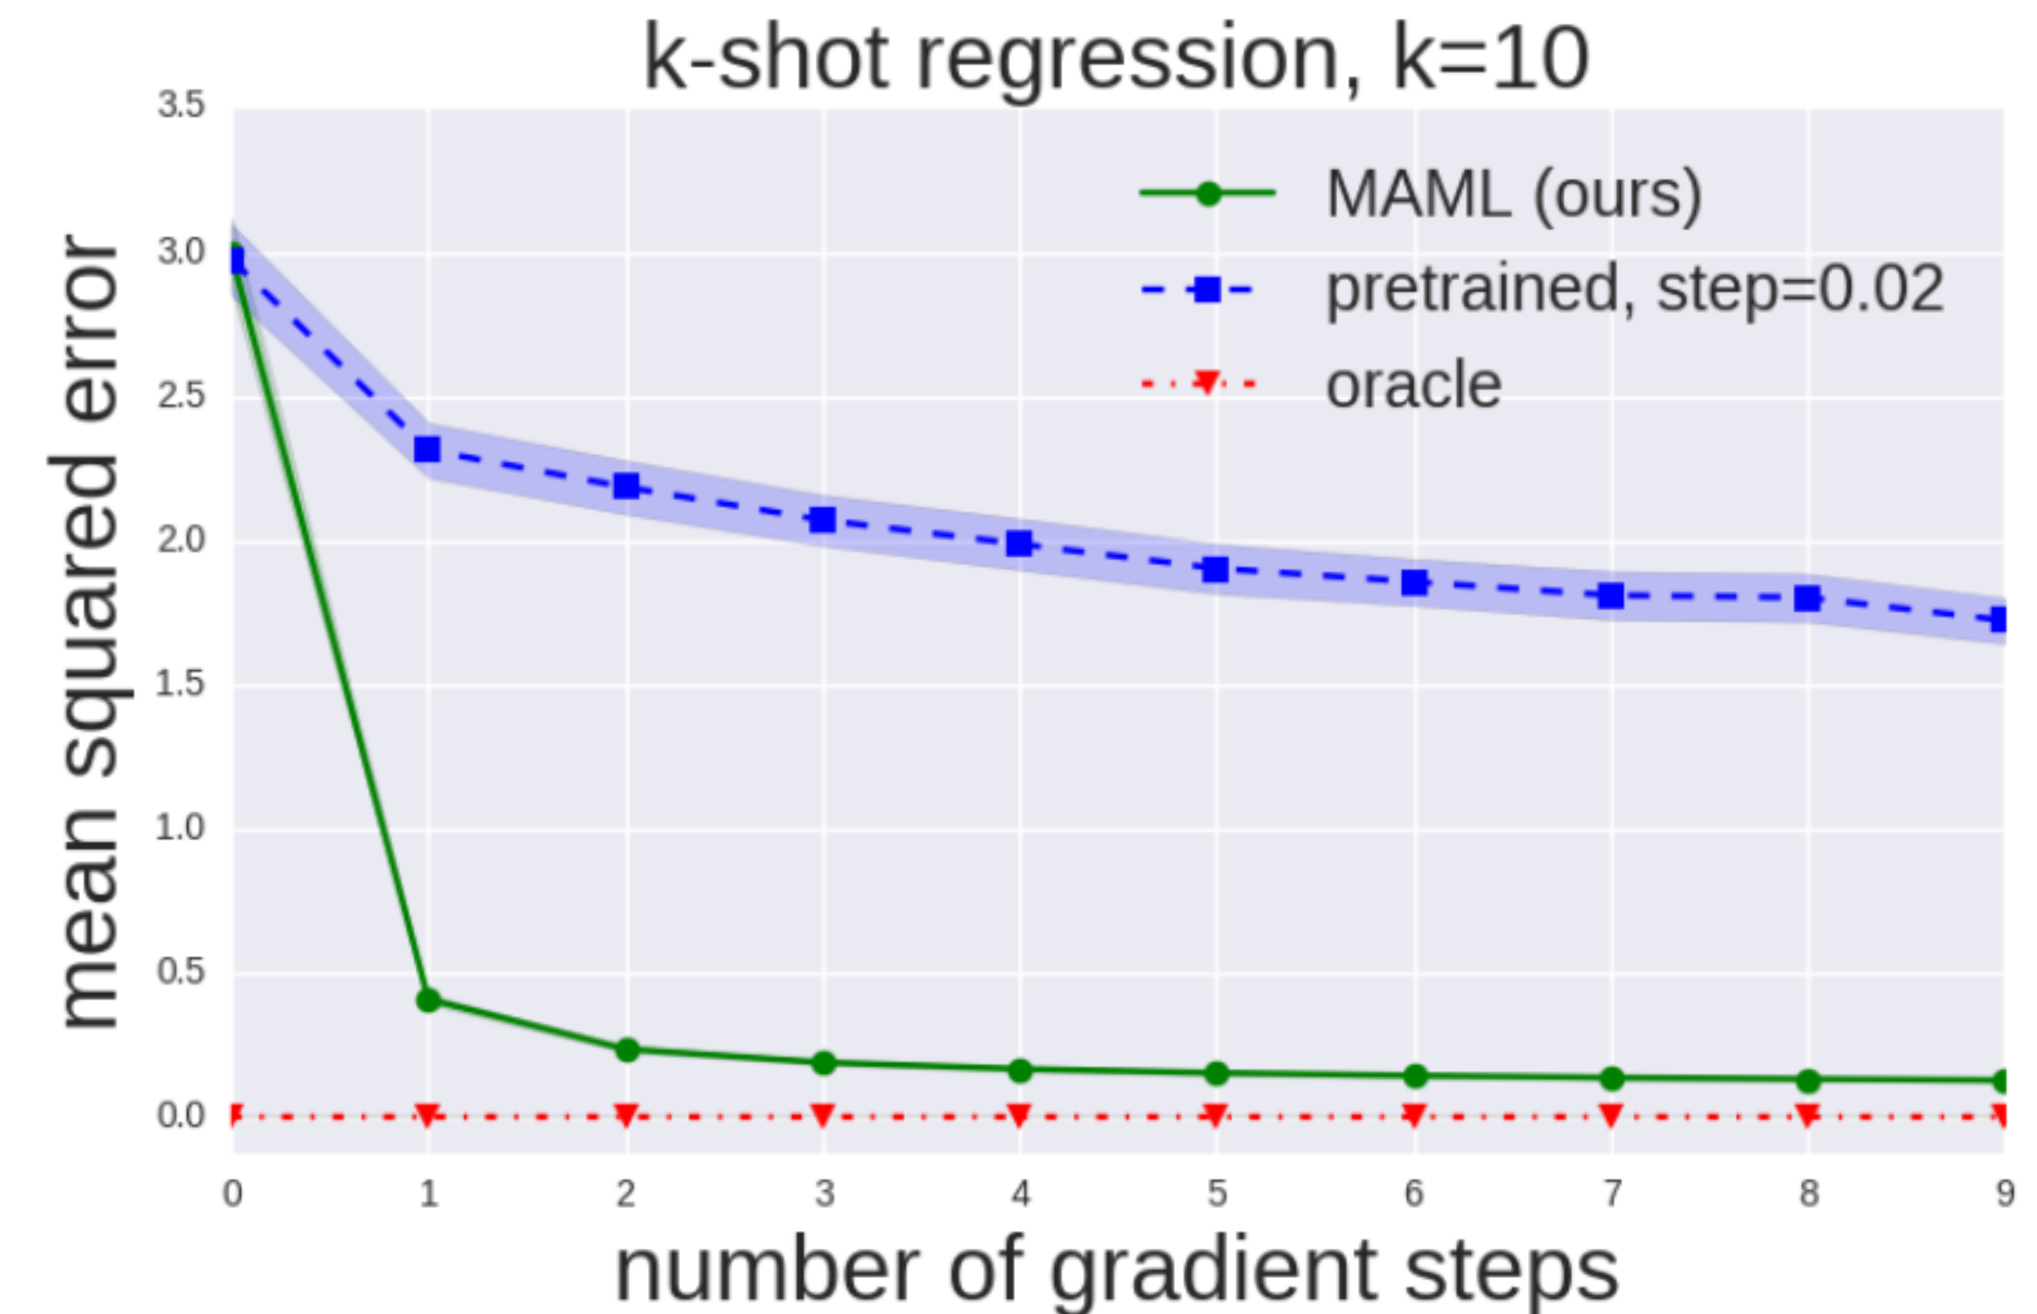
\includegraphics[width=0.4\linewidth]{"C:/Users/dvrch/Desktop/Memoire 2024/Straightforward-Obsidian2Latex/Straightforward-Obsidian2Latex-DV/example_vault/✍Writing/figure blocks/Pasted image 20240609012140.png"}
\caption[]{The caption.}

\label{fig:gradient_steps}
\end{figure}
% End obsidian ref




\subsubsection{With subfigures}

See \Cref{fig:1}.





\begin{itemize}
\item \\twemoji{plus}  Allow user to create more complex configurations
\end{itemize}

% Start obsidian ref:
%figure__block_1\\#\#fig
\begin{figure}[htb]
\centering
\begin{subfigure}[b]{0.5\textwidth}
\centering
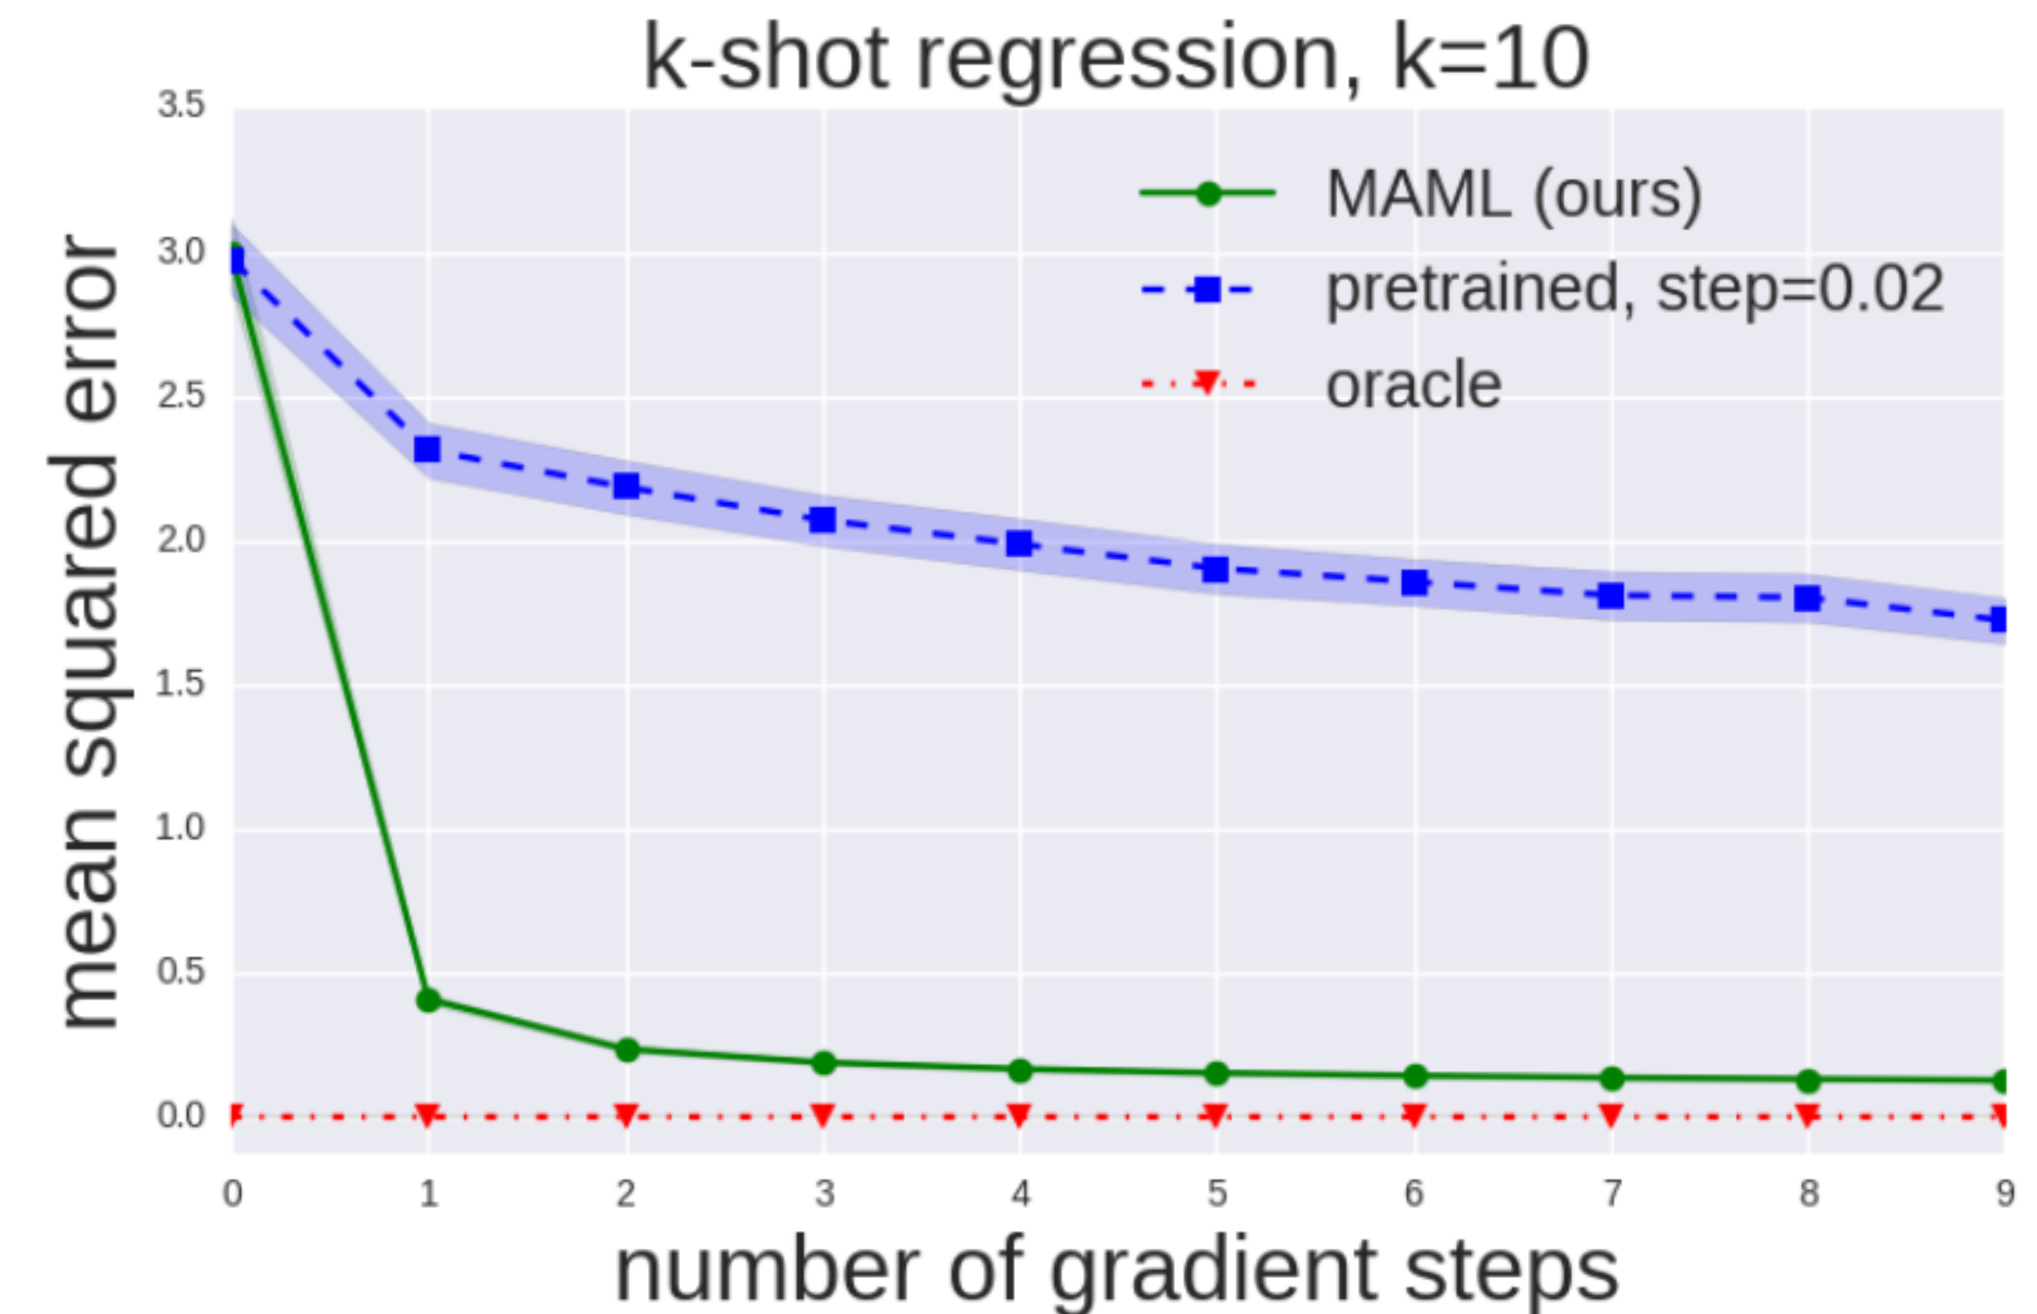
\includegraphics[width=\linewidth]{"C:/Users/dvrch/Desktop/Memoire 2024/Straightforward-Obsidian2Latex/Straightforward-Obsidian2Latex-DV/example_vault/✍Writing/figure blocks/Pasted image 20240609012221.png"}
\caption[]


\end{subfigure}\hfill
\begin{subfigure}[b]{0.5\textwidth}
\centering
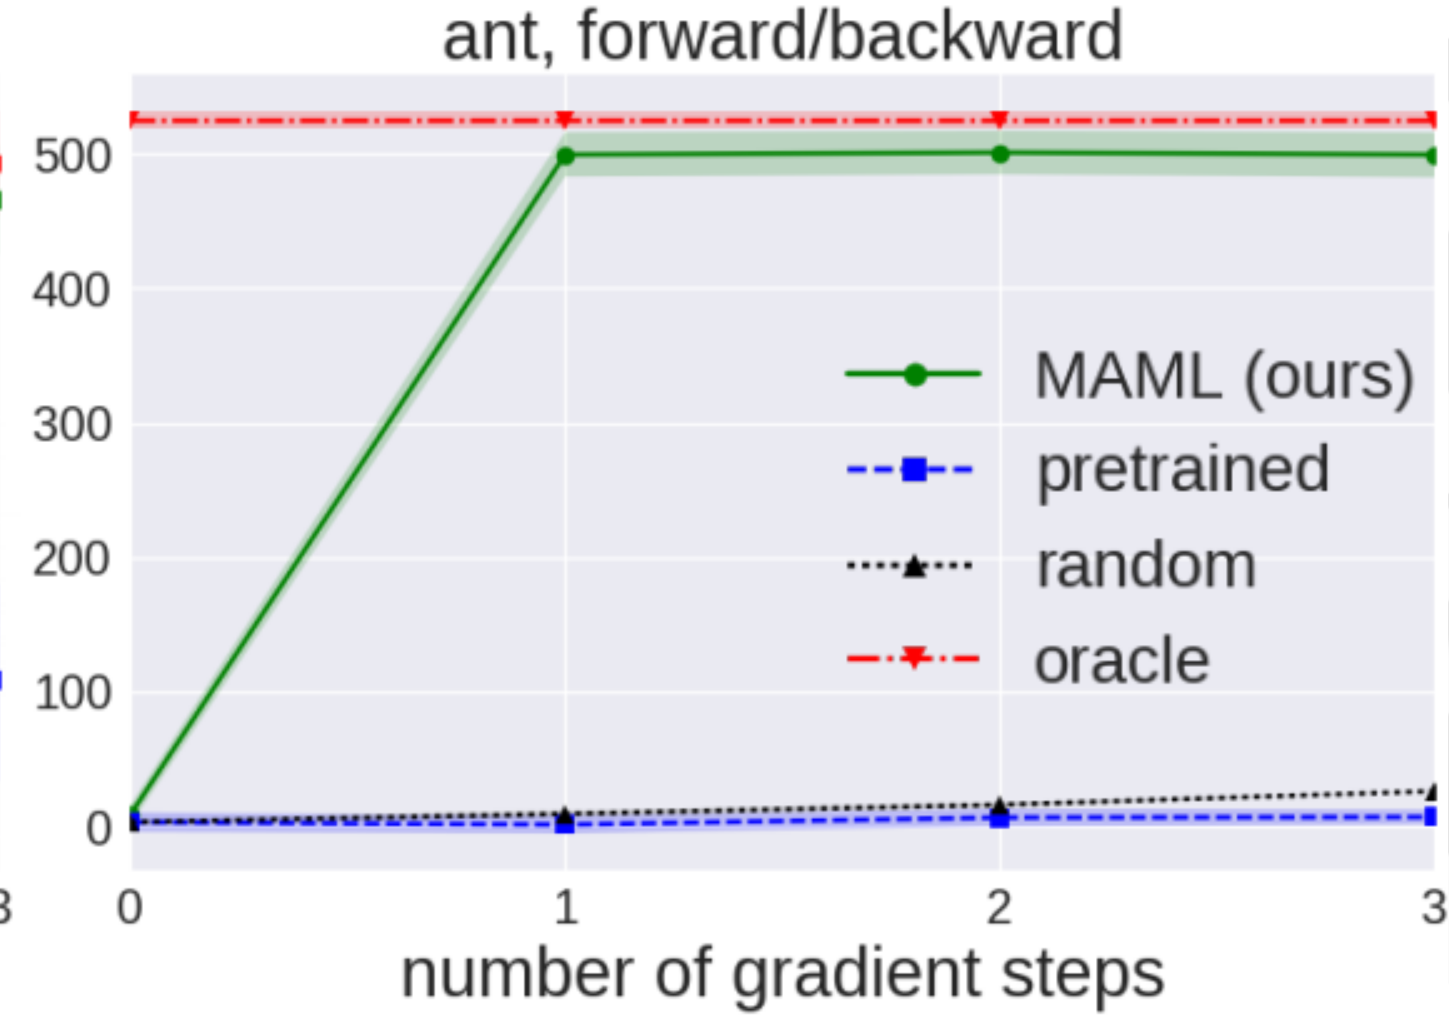
\includegraphics[width=\linewidth]{"C:/Users/dvrch/Desktop/Memoire 2024/Straightforward-Obsidian2Latex/Straightforward-Obsidian2Latex-DV/example_vault/✍Writing/figure blocks/Pasted image 20240609012251.png"}
\caption[]


\end{subfigure}\hfill
\caption{}
\label{fig:1}
\end{figure}

% End obsidian ref






\subsection{Referencing figures}

In \Cref{fig:1}, we can notice that...





\section{Admonition blocks}

If you write admonition blocks, they are translated into something similar in latex.

\textbf{Example}

\begin{tcolorbox}[width=1.0\textwidth,colback={red},title={warning},outer arc=0mm,colupper=white]

This is a warning

\end{tcolorbox}



\begin{tcolorbox}[width=1.0\textwidth,colback={white},title={note},outer arc=0mm,colupper=black]

This is a note

\end{tcolorbox}





\section{Code blocks}

\begin{minted}{python}

print("this is a code block")

print("this is another code block")

\end{minted}



\section{Cross-reference of section}

Check \hyperref[sec:Adding-citations]{this section} (\autoref{sec:Adding-citations}) about adding citations.





\section{\maltese Cross-reference of block}

example



\section{Assume sections from embedded notes}

The sections from embedded notes can assume the hierarchy of the file wherein they are embedded.

\begin{tcolorbox}[width=1.0\textwidth,colback={white},title={note},outer arc=0mm,colupper=black]

Notice in the latex file that the section hierarchy has been modified to adhere to the hierarchy of the file that embeds the note.

\end{tcolorbox}




% Start obsidian ref:
%embedded with sections
\subsubsection{Section 1 of embedded By me}
\paragraph{subsection 1 of embedded} \hspace{0pt} \\
% End obsidian ref




\section{Hyperlinks}

Click \href{https://www.youtube.com/}{here}.





\section{Tables}



See \Cref{tab:1}, \Cref{tab:2}, and \Cref{tab:long}.




% Start obsidian ref:
%table__block_1\\#\#table
%\begin{center}
\begin{table}[ht]
\centering
\caption{Caption of table written in Obsidian}
\label{tab:1}
\begin{tabular}{p{3cm}p{3cm}p{3cm}p{3cm}}
\bottomrule
\textbf{Col1} & \textbf{Col2} & \textbf{Col3} & \textbf{Col4} \\\midrule
a11 & a12 & Some more text & even more text \\
a21 & Equation: $E=mc^{2}$ & Some more textSome more textSome more textSome more textSome more textSome more text & even more text even more text even more text even more text even more text \\
Reference \Cref{eq:1} & 1 & 1 & 1 \\
\hline
\end{tabular}
\end{table}

% End obsidian ref





% Start obsidian ref:
%table__block_2\\#\#table
\newcolumntype{Y}{>{\centering\arraybackslash}X}
%\begin{center}
\begin{table}[ht]
\centering
\caption{Table with customized widths and row color formatting}
\label{tab:2}
\begin{tabularx}{p{1cm}p{1cm}p{5cm}p{3cm}}
\hline
\textbf{Col1} & \textbf{Col2} & \textbf{Col3} & \textbf{Col4} \\
\rowcolor{lightgray}  a11 & a12 & Some more text & even more text \\
\rowcolor{yellow} a21 & Equation: $E=mc^{2}$ & Some more textSome more textSome more textSome more textSome more textSome more text & even more text even more text even more text even more text even more text \\
Reference \Cref{eq:1} & 1 & 1 & 1 \\
\hline
\end{tabularx}
\end{table}

% End obsidian ref





% Start obsidian ref:
%table__block_long\\#\#table
%\begin{center}
\begin{longtable}{p{3cm}p{3cm}p{3cm}p{3cm}}
\caption{A long table. Changed the package in the table file properties}
\label{tab:long}\\
\hline
\textbf{Col1} & \textbf{Col2} & \textbf{Col3} & \textbf{Col4} \\
\hline
\endfirsthead % Use \endfirsthead for the line after the first header
\hline
\endfoot
a11 & a12 & Some more text & even more text \\
a21 & Equation: $E=mc^{2}$ & Some more textSome more textSome more textSome more textSome more textSome more text & even more text even more text even more text even more text even more text \\
Reference \Cref{eq:1} & 1 & 1 & 1 \\
Some more textSome more textSome more textSome more textSome more textSome more text & Some more textSome more textSome more textSome more textSome more textSome more text & Some more textSome more textSome more textSome more textSome more textSome more text & Some more textSome more textSome more textSome more textSome more textSome more text \\
Some more textSome more textSome more textSome more textSome more textSome more text & Some more textSome more textSome more textSome more textSome more textSome more text & Some more textSome more textSome more textSome more textSome more textSome more text & Some more textSome more textSome more textSome more textSome more textSome more text \\
Some more textSome more textSome more textSome more textSome more textSome more text & Some more textSome more textSome more textSome more textSome more textSome more text & Some more textSome more textSome more textSome more textSome more textSome more text & Some more textSome more textSome more textSome more textSome more textSome more text \\
\end{longtable}

% End obsidian ref




\section{Latex commands}

When there is something niche, or some translation functionality that hasn't been developed yet, you can write a latex command within the code-block functionality of Obsidian, and the translator will not touch it. Use the syntax according to the following example:





\lipsum[1-4]




\newpage \n \newpage \n \n\n\n\n\n\bibliographystyle{apacite}
\bibliography{BIBTEX}
\end{document}
